\documentclass{template/openetcs_article}
%\documentclass{article}
%\usepackage[ascii]{inputenc}
%\usepackage[T1]{fontenc}
\usepackage[english]{babel}
\usepackage{amsmath}
\usepackage{amssymb,amsfonts,textcomp}
\usepackage{array}
\usepackage{supertabular}
\usepackage{hhline}
\usepackage{graphicx}
\makeatletter
\newcommand\arraybslash{\let\\\@arraycr}
\makeatother
\setlength\tabcolsep{1mm}
\renewcommand\arraystretch{1.3}
\newcounter{Ilustracin}
\renewcommand\theIlustracin{\arabic{Ilustracin}}
\title{openETCS}

%\setcounter{tocdepth}{3}

\usepackage{hhline}
\usepackage{booktabs}
\usepackage{multirow}
\usepackage{color, colortbl}
\definecolor{myblue}{rgb}{0.6,.6,1}
\definecolor{mydarkblue}{rgb}{0,0,0.5}

\usepackage{hyperref}
\hypersetup{colorlinks=true, linkcolor=mydarkblue, urlcolor=mydarkblue}



% Use the option "nocc" if the document is not licensed under Creative Commons
%\documentclass[nocc]{template/openetcs_article}
\usepackage{lipsum,url}
\graphicspath{{./template/}{.}{./images/}}
\begin{document}
\frontmatter
\project{openETCS}

%Please do not change anything above this line
%============================
% The document metadata is defined below

%assign a report number here
\reportnum{OETCS/WP1/D1.3.1}

%define your workpackage here
\wp{Work-Package 1: ``Management''}

%set a title here
\title{Project Quality Assurance Plan}

%set a subtitle here
%\subtitle{A template for short document. Adapted from report template.}

%set the date of the report here
\date{\today}

%define a list of authors and their affiliation here

\author{Rico Kaseroni}

\affiliation{DB Netz AG\\
  V\"olckerstr. 5 \\
  80939 Munich, Germany}


% define the coverart
\coverart[width=350pt]{openETCS_EUPL}

%define the type of report
\reporttype{Description of work}




%=============================
%Do not change the next three lines
\maketitle
\tableofcontents
%\listoffiguresandtables
\newpage
%=============================

% The actual document starts below this line
%=============================


%Start here




%\begin{document}


\subsection*{Document History}

\begin{flushleft}
%\tablefirsthead{\hline Version & Date & Chapters modified & Reason & Name\\}

\tablehead{\hline \rowcolor{myblue} Version & Date & Chapters modified & Reason & Name\\}

%\tabletail{}
%\tablelasttail{}
\begin{supertabular}{m{1.1cm}m{1.8cm}m{2cm}m{5cm}m{4cm}}
\hline
0.0.0 &
15.11.2012 &
All &
First Steps on frame evaluation &
Rico Kaseroni (DB)

Peyman Farhangi (DB)\\\hline
0.1.0 &
27.11.2012 &
All &
First Steps on Content &
Rico Kaseroni (DB)

Jan Welte (TUB)

Peyman Farhangi (DB)

Matthias Kuhn (DB)\\\hline
0.1.1 &
29.11.2012 &
All &
Optimaziation of document structure, Revision of Chapters according to EN 50128, Merging with project specific tasks &
Stephan Jagusch (AEbt)

Rico Kaseroni (DB)

Cyril Cornu (All4tec)\\\hline

0.2.0 &
30.11.2012 &
Baseline Requirements for certification  &
Extention of Chapter according to EN 50128 &
Jan Welte (TUB)

Rico Kaseroni (DB)\\\hline
0.3.0 &
19.12.2012 &
All &
Extention of Chapter 

0, 1, 2, 3 &
All4Tech, DB, SQS\\\hline
0.4.0 &
11.01.2013 &
All &
Extention to existing and further Chapters  &
All4Tech, DB, SQS\\\hline
0.6.0 &
28.01.2013 &
All &
IP Clean &
Rico Kaseroni (DB)

Cyril Cornu (All4tec)\\\hline
0.6.1 &
29.01.2013 &
Scrum &
Contribution &
Bernd Hekele (DB)\\\hline
0.7.0 &
01.02.2013 &
All &
More Content &
Rico Kaseroni (DB)\\\hline
0.8.0 &
02.02.2013 &
All &
Jungle Content -{\textgreater} Smooth &
Rico Kaseroni (DB)\\\hline
0.9.0 &
06.02.2013 &
All &
Review on 0.8.0 Version &
Dr. Hase (DB)\\\hline
0.9.1 &
07.02.2013 &
Scrum &
Optimization &
Bernd Hekele (DB)\\\hline
0.9.2 &
07.02.2013 &
All &
Restructuring  &
Rico Kaseroni (DB)\\\hline
0.9.3 &
11.02.2013 &
1-, 2-, Last Chapter Annex A and C  &
Graphic Figure 1, Definition of openETCS Process IP clean Job &
Rico Kaseroni (DB)\\\hline
0.9.4 &
12.02.2013 &
All &
Optimization  &
Rico Kaseroni (DB)\\\hline
0.9.4.5 &
15.02.2013 &
Chapter2 &
System Testing &
Rico Kaseroni (DB)\\\hline
0.9.4.6 &
15.02.2013 &
ALL &
Optimization  &
Rico Kaseroni (DB)\\\hline
0.9.5 &
22.02.2013 &
ALL &
Restructuring \& Optimization  &
Rico Kaseroni (DB)\\\hline
0.9.5.1 &
01.03.2013 &
ALL &
LaTeX conversion &
Peter Mahlmann (DB)\\\hline
0.9.5.2 &
04.03.2013 &
ALL &
LaTeX Optimization  &
Rico Kaseroni (DB)\\\hline
\end{supertabular}
\end{flushleft}


\newpage



\section{Introduction}
This software quality Assurance Document will cover the standards, processes, and procedures for the openETCS project in order to achieve a correct implementation.


\subsection{openETCS Project Goals}
The OpenETCS main objective is the development of an ``open proofs'' platform that integrates technologies from various stakeholders and enables the use of formal verification techniques in order to dramatically improve the software quality for embedded control systems in terms of reliability, maintainability, safety, and security.

Following are openETCS Goals defined based on Project Co-operation Agreement:

\begin{enumerate}
\item Creating a \emph{formal specification} of the ETCS OBU functionality according to UNISIG Subset 026

\item An \emph{executable software package} generated from the formal specification and a \emph{non-vital implementation of that software} for laboratory test, simulation and reference purposes

\item A \emph{tools chain} supporting both previous bullet points including code, test case and document generation meeting CENELEC EN50128:2011 (T3) requirements and certifiable for SIL4 software applications for signalling equipment (Certification itself is not part of the project)
\end{enumerate}


In summary, the ``openETCS'' approach is based on a relatively new ``open proofs'' concept using formal methods and extending open source principles to tools and safety case documents. Thus both, economical and technical problems are addressed equally by cost sharing effects and broadening the peer-to-peer review basis, taking into account latest technical standards (e.g. EN50128:2011) for tools and software life cycle management.


\subsection{Field of application -- Context}
\subsubsection{Context}
Even though all new main line railway infrastructure installations are required to be equipped with ETCS components, the overwhelming part of lines are still equipped with national legacy signalling and train control and protection systems with variety of technologies. For a unified European rail system it is very costly to maintain this diversity of signalling systems.

Therefore, ETCS is intended to replace national legacy signalling and train control systems, but has to work in parallel with those old systems for many years to come, since a complete migration to ETCS will take several decades. ERTMS is the only ``Standard'' for signalling systems with more than one supplier on the market due to open specification, while other systems are proprietary, that means a particular system is only available from mostly one single source. Nevertheless ERTMS will only be competitive in the world market if the cost total level for the system is becoming more competitive with alternative systems.

\begin{figure}
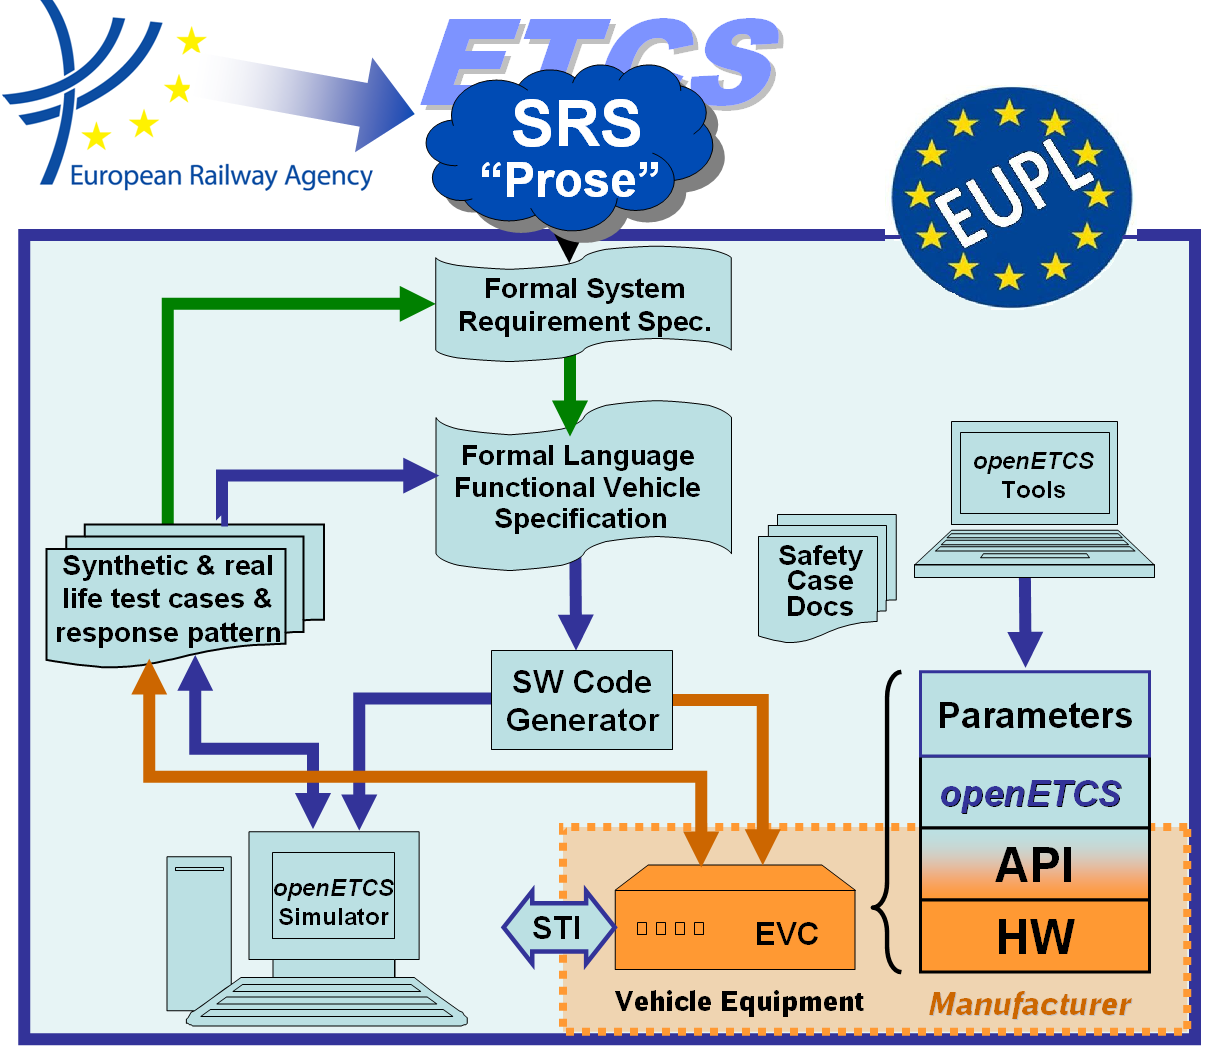
\includegraphics[width=\textwidth]{./figures/openETCS_EUPL.png}
\caption{OpenETCS Scope of Work}
\end{figure}

The key element for improving that situation seems to be a greater degree of standardization for: Hardware, software, methods and tools in combination with formal methodology and modeling technique, applying open source license schemes to promote and encourage EU wide cooperation. The proposed open source approach is utilizing concepts from the automotive and aviation industry, not only covering the embedded control software of the ETCS onboard unit itself, but including all tools and documents in order to make the entire product life cycle as transparent as possible and make it comprehensible for third parties. Making the proof of safety open to the entire professional world has been called ``open proof'' and is new to the railway sector.


\subsubsection{Technology}
The EVC (European Vital Computer) is the heart of the ERTMS onboard system. This safety computer implements the functions of the SRS subset 026 of UNISIG (for SRS versions beginning with baseline 3, published by ERA) in order to guarantee the safety of the train movements.

The OpenETCS scope of application is related to the only EVC part of whole ERTMS system. The Track-side part of the ETCS (the Radio Based Control) is excluded from the project activities, and only considered through its interfaces with the On-Board part of ETCS.

First Focus of the openETCS project is the implementation and test of processes and tools being the basis for a high quality EVC build.

Second focus of the openETCS project is the use of open source concepts, based on the Eclipse ideas [ECLIPSE] under EUPL licensing.

Third focus of the openETCS project is the introduction of agile software development procedures. Agile development is introduced with SCRUM methodology. SCRUM is well known and well documented in other parts of the software industry. 

For detailed information, please refer to e.g., [SCRUM]. We assume the reader is familiar with Scrum methodology (if not, have a look in one of the books available or ask for training). The project quality assurance plan will not describe Scrum in detail. In this document, we only define relevant aspects related to processes and quality. This is mainly limited to the description of how Scrum is implemented in the project organization.

Typically, agile development goes in hand-in-hand with lean management , i.e., restructuring of the organization. However, the change of the organization is not in the focus of this project. 

Last but not least, the approach of Formal Methods is in the focus of this document [FM].



\subsection{Eclipse}
It is the largest open source project. At the same time there are certain behavior which describe the success of Eclipse project. We will follow these rules for openETCS with the scope of possibilities and guidelines of CENELEC specially EN50128 from June 2011.


\subsection{Creation}
This Quality Assurance Plan addresses the first attempt to adapt the well established Eclipse process in a way that CENELEC requirements -specially EN 50128 (Ref [N01])- are satisfied on achieving the goals of openETCS project. Eclipse process is optimized for the open source development which we are aiming as strategy for openETCS project.

This Quality Assurance Plan is created by the Project Quality Assurance Manager in co-operation with openETCS partners and members. It will be submitted to all openETCS partners for review, to Work Packages managers for approval and to the openETCS project manager to validate this document.

Updating and diffusion of this document is on project quality assurance manager responsibility. They has to be approved by project manager before diffusion.

The main document diffusion issues are:
\begin{itemize}
\item Main project and features improvements or evolutions
\item At least once per year, following Project quality audit
\end{itemize}
These revisions are summarized in the Document History. You will find this document under  [Link will be delivered]


\section{Project Life Cycle}
Projects go through six distinct phases. The transitions from phase to phase are open and transparent public reviews.

\begin{figure}
\centering
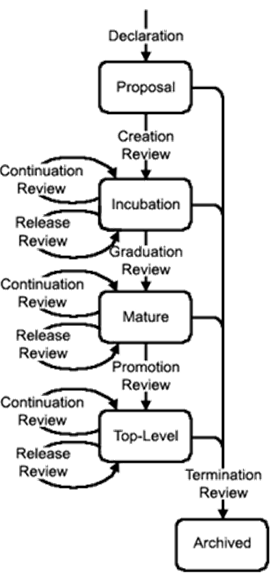
\includegraphics[width=.4\textwidth]{./figures/lifecycle.PNG}
\caption{Project lifecycle}
\end{figure}
  

\section{Process}
In framework of Open ETCS project, a Safety certified SIL4 Software has to be supplied, according to the EN50128 standard. The software regarded is the one embedded on the On-Board part of the ETCS system: the EVC.

Development process and its activities are described in this Software Quality Assurance Plan. This document aims at identify, supervise and control all these activities. It provides the quality process and approach needed to avoid developing process hazards, and assures compliancy with the EN50128 requirements.

All documentation delivered in the framework of this software development needs to be compliant with EN 50128 standard (Ref [N01]).



\subsection{Process description}
This is the description of the Development Process for the openETCS project. In particular, it describes how participants influence, and collaborate with Projects to achieve these openETCS purposes. The process follows the template of the Eclipse development process\footnote{\url{http://www.eclipse.org/projects/dev\_process/development\_process\_2011.php}}, including minor adaptations.

The openETCS project is a vendor-neutral, open development project supplying methods, methodologies, tools, frameworks, specifications and implementations of ETCS onboard units and related components. openETCS software are extensible in that their functionality is accessible via documented programmatic interfaces. The purpose of the openETCS project, is to advance the creation, evolution, promotion, and support of work products related to openETCS and to cultivate both an open source community and an ecosystem of complementary products, capabilities, and services. 

An Open Source Project needs strong governance because no traditional management structure can be conducted for that. During the last decade there has been an evolution in OSS IT industry. The most important development is ``Eclipse''. Unfortunately CENELEC is not affected by this evolution. Therefore we need a further development of those requirements by looking into the ``intention and suspected objectives inside CENELEC'' which should be independent from specific legacy styles of management.


\subsubsection{Process Requirements by CENELEC}
In this document we will describe what exactly are the minimum requirements of CENELEC and how we can conduct them in openETCS project.


\subsubsection{openETCS Process Definition}
Following points describe the guiding principles used in developing this Development Process.


\paragraph{Open Source Rules of Engagement}
Open - openETCS is open and provides the same opportunity to all. Everyone participates with the same rules; there are no rules to exclude any potential contributors which include, of course, direct competitors in the marketplace.

Transparent - Project discussions, minutes, deliberations, project plans, plans for new features, and other artifacts are open, public, and easily accessible.

Meritocracy - openETCS is a meritocracy. The more you contribute the more responsibility you will earn. Leadership roles in openETCS are also merit-based and earned by peer acclaim.

\paragraph{openETCS Ecosystem}
openETCS is the sum of its parts (all of the Projects), and Projects should strive for the highest possible quality in documents, extensible frameworks, exemplary tools, transparent processes, and project openness.

It is the responsibility of the project participants to ...cultivate...an ecosystem of complementary products, capabilities, and services.... It is therefore a key principle that the openETCS Development Process ensures that the projects are managed for the benefit of both the open source community and the ecosystem members. To this end, all openETCS projects are required to:
\begin{enumerate}
\item communicate their project plans and plans for new features (major and minor) in a timely, open and transparent manner;
\item create high-quality and understandable documents, which follow standards and common vocabulary;
\item create platform quality frameworks capable of supporting the building of commercial grade products on top of them; and
\item ship extensible, exemplary tools which help enable a broad community of users.
\end{enumerate}


\paragraph{Three Communities}
Essential to the Purposes of openETCS is the development of three inter-related communities around each Project:

Contributors and Committers - a thriving, diverse and active community of developers is the key component of any openETCS Project. Ideally, this community should be an open, transparent, inclusive, and diverse community of Committers and (non-Committer) Contributors. Attracting new Contributors and Committers to an open source project is time consuming and requires active recruiting, not just passive ``openness''. The Project Leadership must make reasonable efforts to encourage and nurture promising new Contributors.

Projects must have diversity goals to ensure diversity of thought and avoid relying on any one company or organization. At the same time, we acknowledge that enforcing a particular diversity metric is a poor way to achieve these goals; rather we expect the project leadership to help the diversity evolve organically.

Diversity is a means to an end, not an end in itself, thus diversity goals will differ by project based on the other accomplishments of the project(s).

Projects are required to explain their diversity efforts and accomplishments during Reviews.

Users - an active and engaged user community is proof-positive that the Project's exemplary tools are useful and needed. Furthermore, a large user community is one of the key factors in creating a viable ecosystem around an openETCS project, thus encouraging additional open source and commercial organizations to participate. Like all good things, a user community takes time and effort to bring to fruition, but once established is typically self-sustaining.

Adopters - an active and engaged adopter developer community is the only way to prove that an openETCS project is providing extensible frameworks and extensible tools accessible via documented APIs. Reuse of the frameworks within the companies that are contributing to the project is necessary, but not sufficient to demonstrate an adopter community. Again, creating, encouraging, and nurturing an adopter community outside of the Project's developers takes time, energy, and creativity by the Project Leadership, but is essential to the Project's long-term open source success.

The openETCS community considers the absence of any one or more of these communities as proof that the Project is not sufficiently open, transparent, and inviting, and/or that it has emphasized tools at the expense of extensible frameworks or vice versa.


\paragraph{Clear, Concise, and Evolving}
It is an explicit goal of the Development Process to be as clear and concise as possible so as to help the Project teams navigate the complexities, avoid the pitfalls, and become successful as quickly as possible.

This document imposes requirements and constraints on the operation of the Projects, and it does so on behalf of the openETCS community. It is an explicit goal of the Development Process to provide as much freedom and autonomy to the Projects as possible while ensuring the collective qualities benefit the entire openETCS community.


Similarly, this document should not place undue constraints on Project Leads, the Project Management Board (PMB) or committers that prevent them from governing the process as necessary. We cannot foresee all circumstances and as such should be cautious of being overly prescriptive and/or requiring certain fixed metrics.

The frameworks, documents, specifications, tools, projects, processes, community, and even the definition of Quality continues to, and will continue to, evolve. Creating rules or processes that force a static snapshot of any of these is detrimental to the health, growth, and ecosystem impact of openETCS.

Part of the strength of this document is in what it does not say, and thus opens for community definition through convention, guidelines, and public consultation. A document with too much structure becomes too rigid and prevents the kind of innovation and change we desire for openETCS. In areas where this document is vague, we expect the Projects and all participants to engage the community-at-large to clarify the current norms and expectations.


\subsection{Committers assignment and responsibilities}

This part of the document makes the connection between the Project Tasks defined within the different Work packages, and the Software key roles identified in the CENELEC Standard (Ref [N01]).

As OpenETCS is an open source project, there is not just one people personally assigned to one Software Key Role, but many different committers and stake holders. Moreover, according to the agile needs, these people can change during the Development Process.

According to these reasons, the Project Key Roles are assigned to well identified project tasks, and not to the tasks or Work Packages leaders. The detail of assignments, roles and responsibilities of each committer along the whole Software Development Life cycle are detailed in a separated document: the Assignment Configuration Management (Ref [N{\dots}]).

\subsection{Committers Competencies}

According to the EN50128 Standard, all personnel who have responsibilities for the software are organized, empowered and capable of fulfilling their responsibilities. Moreover, these people shall be competent to discharge those responsibilities by demonstrating the ability to perform relevant tasks correctly, efficiently and consistently to a high quality and under varying conditions.

As many committers and contributors are involved in the Open ETCS Project, the people responsible or involved in a project task defined as Key Software Role, have to prove that he has the needed skills to perform this task in accordance with the CENELEC requirements. Indeed, this personnel assigned to the roles involved in the development or maintenance of the software shall be named and recorded.

Therefore, this chapter encompasses 3 different parts:
\begin{itemize}
\item The Needed Competencies Matrix. Based on the Open ETCS Work Packages / Tasks structure, this table describes which competencies are needed for each stake holder depending on its role according to the standard.
\item The Actual Competencies Matrix. Still based on the Open ETCS Work Packages / Tasks structure, this table summarizes the actual competencies of each stake-holder.
\item Deduced from the 2 previous competencies, a Training Plan for Project Stake Holders is defined. This plan aims at allow people responsible for EN50128 compliant activities, to reach the skill and competencies level required for EN50128 standard compliancy.
\end{itemize}

\subsubsection{Required Competencies Matrix}

According to CENELEC Requirements, each Committer shall demonstrate their ability to perform relevant Software Key tasks properly, efficiently and consistently to a high quality and under various conditions.

According to CENELEC Requirements, the Task Leaders that are managing software key tasks shall manage these required Competencies for all involved committers. Each competencies and skills needed for each Software Key Role are described in Annex B - Ref [N01].

The Required Competencies Matrix has to be fulfilled by each Task Leader for each Tasks related to a Key Software Role according to the CENELEC requirements. A Matrix template is provided in Annex A.


\subsubsection{Actual Competencies Matrix}
According to the OpenETCS project structure, all involved committers competencies and skills are summarized in the actual competencies matrix, provided in Ref [N01].

Documented evidence of personnel competence, including technical knowledge, qualifications, relevant experience and appropriate training, shall be maintained by the supplier's organization in order to demonstrate appropriate safety organization and accordance to the CENELEC requirements. This documentation activity has to be managed and supervised by the relevant appropriate task leader.


\subsubsection{Training plan}
Deduced from the two previous parts, and according to the Ref [N01] - {\S}5.2.2.4, a training plan is created, in order to provide to each committer the needed competencies and skills.

The Training Plan has to be managed by each Task Leader for each Tasks related to a Key Software Role according to the CENELEC requirements.

\begin{figure}
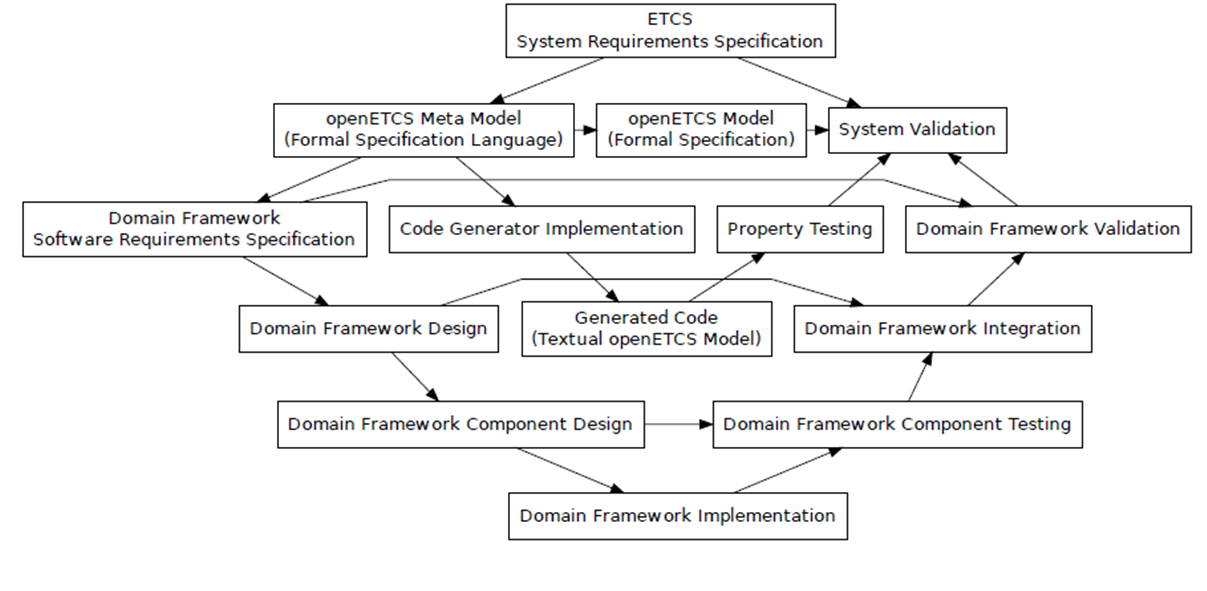
\includegraphics[width=\textwidth]{./figures/lifecycle3.PNG}
%\caption{Training plan}
\end{figure}


\subsubsection{Open ETCS Software life cycle based on Eclipse in accordance to CENELEC EN50128}


Eclipse Lifecycle has following strategy. It starts in July. It goes for 6 weeks. Within these 6 weeks will have every 2 weeks a Scrum Sprint which means 3 sprints within this 6 weeks. At the end of 6 weeks there will be an interim release. Afterwards the next 6 weeks starts in order to achieve the next interim release. In total we will have 8 times of these 6 weeks. At the end of 8 times each 6 weeks we will have a 4 weeks preparation phase in order to have a proper Major Release. In Total a Major release take one year.  

Now in order to be in compliance with CENELEC, we have to abide by to the rules in Chapter 7 of EN50128 in his lifecycle strategy.





 
\subsection{Documentation}

\subsubsection{Documentation and control}
This paragraph describes the different quality assurance related documents that have to be issued within each Work Package and task of the project.

This task is currently worked out, and a final version of the Input/output of each Tasks and WorkPackages will be provided after the 5th February.


\begin{tabular}{|m{2.25cm}|m{7cm}|m{1cm}|m{1cm}|m{1cm}|m{1cm}|}
\hline 
\rule[-1ex]{0pt}{2.5ex} \multirow{2}{*}{Doc. ref.} & \multirow{2}{*}{Description of the document} & \multicolumn{2}{c|}{Issued within} & \multicolumn{2}{c|}{Destinated to} \\ 
\hhline{~~----}
  &  & WP & Task & WP & Task \\ 
\hline 
\rule[-1ex]{0pt}{2.5ex} \centering O$_1$\_WP$_2$\_T$_{2\_2}$ & Report of existing methodologies in signaling or similar industrial contexts (State-of-the-art) & WP$_2$ & T$_{2\_2}$ &  &  \\ 
\hline 
 O$_2$\_WP$_2$\_T$_{2\_2}$ & Set of requirements to be fulfilled according to CENELEC standards (state-of-the-art) & WP$_2$ & T$_{2\_2}$ &  &  \\ 
\hline 
\end{tabular} 



\subsubsection{Documentation Quality}
The quality assurance activities, actions and documents shall be specified or referenced in this document. A Software Quality Assurance Verification Report shall be written, under the responsibility of the Verifier, on the basis of all the input documents available from the project.

For each document issue, an inspection process shall be realized according to the following steps:

\begin{itemize}
\item A first draft version of the document is written by a person part of the relevant task committers;
\item Then, another person, competent and independent from the author, will review the document through a revision sheet encompassing all the remarks gathered during the document review;
\item Once the review phase done, the revision sheet is sent to the author, who considers or not the remarks, and justifies their acceptance or refusal;
\item Once the document has been updated by the author, the document has to be sent back to the reviewer, in order that he checks the remarks acceptance or refusal, and their justification. If the author's answers are to be discussed again;
\item The document can be issued in an official version and distributed once all remarks have been closed.
\end{itemize}


The document author shall establish, document and maintain procedures for control of the external suppliers, including methods and relevant records to ensure that the requirements provided to the External Customer are adequate and complete.


\subsubsection{Traceability}
In order to comply with a SIL4 level according to the CENELEC standard, the following requirements have to be respected: {\S}5.3.2.8, {\S}5.3.2.9, {\S}5.3.2.10, {\S}5.3.2.13, {\S}5.3.2.14.


\subsubsection{Tracking and tracing of deviation}
In order to comply with a SIL4 level according to the CENELEC standard, the following requirements have to be respected: {\S}6.5.4.5, {\S}6.1.4.5, {\S}6.2.4.13, {\S}7.7.4.8, {\S}7.7.4.10.


\subsubsection{Documentation Structure for the whole Project}
The structure of Documentation has to be defined. We have to analyze and follow the way and approach of Eclipse Documentation. 

\subsubsection{Documentation Labeling and the Structure of File Naming}
A suggestion of Sylvain Baro is under discussion.

\subsubsection{State of Documentation}
It is important to underline the state of every Document. If it is in incubation phase , it has to be labeled for that. Here we will describe the list of states in which a Document can go through.


\subsection{Development process}
This part gives an overview of each Work Packages and Tasks content, the input criteria and conditions to start the relevant activities, and the document to be issued. It describes precisely the Software Quality Assurance within the OpenETCS project, and has a project management aspect from a quality point of view (Gant scheduling, critical path etc{\dots})


\subsection{The list of recommended Plans}
Following Plans will enhance the quality of openETCS project and some of them are highly recommended in CENELECT Ref [N01].
\begin{itemize}
\item Software Configuration management Plan
\item Maintenance Plan
\item Validation Plan
\item Verification Plan
\item System Testing plan  
\item Implementation Plan
\item Software deployment Plan
\item Training Plan
\end{itemize}

\subsection{System Testing}
System Testing affects the whole system. System testing of openETCS has to be conducted on a complete, integrated system to evaluate the system's compliance with its specified~requirements. System testing is performed on the entire system in the context of a~Functional Requirement Specification and a~System Requirement Specification. This includes None Functional, Cross Functional, boundaries, Stress and Performance, Integration and Regression Testing. System testing elaborates not only the design, but also the behavior and even the expectations of the initial idea.

In order to have a high quality System Testing, we have to create a System testing plan. 

\subsection{Methods, measures and tools for quality assurance}
All Methods, measures, use of tools and overall requirements for a SIL4 quality assurance are given in Annex A.3 - Ref [N01]

This chapter is structured according to the Software lifecycle phases. (See This document 2.4.4). The Details of methods, measures, tools, and the Overall Software Test Specification will be precisely described in the V\&V plan (Ref [{\dots}.]).


\subsubsection{Software Requirements Specification}
This activity is supposed to describe a complete set of requirements for the software meeting all System and Safety Requirements and provide a comprehensive set of documents for each subsequent phase.

The detail of Input and Output document expected for this Phase is given in EN50128.

All Software Design and Implementation requirements for a SIL4 Software are given in - Ref [N01] CENELEC EN50128


\subsubsection{Architecture and design phase}
This activity is supposed to develop a software architecture that achieves the requirements of the software, and that ensure that the resultant system and its software will be readily testable from the outlet. 

The detailed objectives, and the input/output documents needed are detailed in EN50128.

All architecture and design phase requirements for a SIL4 Software are given in Annex A.4 - Ref [N01].


\subsubsection{Component design phase}
This activity is supposed to develop a software component design that achieves the requirements of the Software Design Specification to the extent required by the software safety integrity level.

The detailed objectives, and the input/output documents needed are detailed in EN50128. The Software Component Design Verification Report has to be issued within the task T4.3, as part of the V\&V phase (described in the EN50128).

All Component design requirements for a SIL4 Software are given in Annex A.4 - Ref [N01].


\subsubsection{Component Design Verification}
This activity is supposed to achieve the overall Component Design Verification. The Software Component Design Verification Report shall be written in accordance with the generic requirements established for a Verification Report.

The detailed objectives, and the input/output documents needed are detailed in EN50128.

All Component Design Verification requirements for a SIL4 Software are given in Annex A.5 - Ref [N01].

The overall Validation and Verification phases are detailed in the V\&V plan (ref [{\dots}]).


\subsubsection{Component Testing and Integration}
\paragraph{Component Testing}
This activity is supposed to test the component and the implementation such as described in previous part.

The detailed objectives, and the input/output documents needed are detailed in Chapter 6  {}- Ref [N01].

All Component testing requirements for a SIL4 Software are given in Annex A.7 - Ref [N01].

\paragraph{Component Integration}
This activity is supposed to achieve software which is analyzable, testable, verifiable and maintainable. Component testing is also included in this phase.

The detailed objectives, and the input/output documents needed are detailed in EN50128.

All Component integration requirements for a SIL4 Software are given in Annex A.6 - Ref [N01].

\paragraph{Software Validation}
This activity is supposed to achieve the validation of the source code. The Software Source Code Verification Report shall be written in accordance with the generic requirements established for a Verification Report.

The detailed objectives, and the input/output documents needed are detailed in EN50128.

The overall Validation and Verification phases are detailed in the V\&V plan (ref [{\dots}]).


\paragraph{Software Verification}
This activity is supposed to examine and arrive at a judgment based on evidence that output items (process, documentation, software or application) of a specific development phase fulfil the requirements and plans with respect to completeness, correctness and consistency. These activities are managed by the Verifier.

The detailed objectives, and the input/output documents needed are detailed in EN50128.

The overall Validation and Verification phases are detailed in the V\&V plan (ref [{\dots}]).The Software Quality Assurance Verification Report requirements are also described in this document.

All Software Verification requirements for a SIL4 Software are given in Annex A.7 - Ref [N01].


\paragraph{Coding Standards}
All Software Verification requirements for a SIL4 Software are given in Annex A.12 - Ref [N01].


\subsection{Traceability of Requirements}
According to EN50128 Standard, the Traceability to requirements shall be an important consideration in the validation of a safety-related system and means shall be provided to allow this to be demonstrated throughout all phases of the lifecycle.

Within the context of this European Standard, and to a degree appropriate to the specified software safety integrity level, traceability shall particularly address:
\begin{itemize}
\item traceability of requirements to the design or other objects which fulfil them,
\item traceability of design objects to the implementation objects which instantiate them,
\item traceability of requirements and design objects to the tests (component, integration, overall test) and analyses that verify them.
\end{itemize}
The overall traceability and documentation requirements are detailed in the Configuration Management plan (ref [{\dots}]).


\subsection{Quality Assurance Standards beside CENELEC }
Following standards have to be considered beside CENELEC,
\begin{itemize}
\item ISO Standards
\item TSI Guide lines and Standards
\item ERA Guide lines and Standarda
\end{itemize}


\subsection{Tool Chain and related Releases}
Regarding toolchain we will have the Ecosystem approach. 

https://github.com/openETCS/toolchain

Regarding Release we will consider the Eclipse approach.


\subsection{Release Train}
The understanding, managing and labeling of Release Train has to be defined. This point is mandatory to be elaborated related to the structure of Release Train of Eclipse project.


\subsection{Github Structure, Project and File Labeling}
Gitgub structure have to abide by to certain rules which most likely comes from Eclipse.

The whole labeling of project and related file have to go through certain criteria. Like starting with a Capital letter, x times letters, y times digits and so on and so far. The scope of the definition of labeling has to be discussed very soon.


\subsection{Organizations and Logos in Documentation}
The logo of such organization like ITEA2 has to be considered in openETCS Documentation. On fronpage as well as certain other places an evaluation is needed to find out which logos, from which organization. On one side we have to consider the permission issue and on the other side we have to show the appreciation on every type of participation. 



\subsection{Quality assurance measures}
Subjects like Formal Methods and Formal Proof, ISO 9126, Open Source Rules, Coaching and mentoring activities, Training,  Validation and Verification, Feed back and Reports, Corrective actions to problem reporting, Guidelines on Development Process, Project Lifecycle, Reviews, Inspections, Releases, Grievance Handling , Documentation and Structure contribute to Quality assurance measures.


\subsubsection{ISO 9126}
ISO 9126 addresses respectively, the following subjects: quality model; external metrics; internal metrics; and quality in use metrics. 

ISO 9126-1 represents the latest (and ongoing) research into characterizing software for the purposes of software quality control, software quality assurance and software process improvement.

The ISO 9126 documentation itself, from the~official ISO 9126 documentation, can only be purchased and is subject to copyright.

The ISO 9126-1 software quality model identifies~6 main quality characteristics, namely:
\begin{itemize}
\item Functionality
\item Reliability
\item Usability
\item Efficiency
\item Maintainability
\item Portability
\end{itemize}


\paragraph{Functionality}

Functionality is the essential purpose of any product or service. The more functions a product has, the more complicated it becomes to define it's functionality. For software a list of functions can be specified.


\paragraph{Reliability}

Once a software system is functioning, as specified, and delivered the reliability characteristic defines the capability of the system to maintain its service provision under defined conditions for defined periods of time. One aspect of this characteristic is~fault tolerance~that is the ability of a system to withstand component failure. For example if the network goes down for 20 seconds then comes back the system should be able to recover and continue functioning.~

\paragraph{Usability}
Usability only exists with regard to functionality and refers to the ease of use for a given function. The ability to learn how to use a system (learnability) is also a major sub characteristic of usability.~


\paragraph{Efficiency}

This characteristic is concerned with the system resources used when providing the required functionality. The amount of disk space, memory, network etc. provides a good indication of this characteristic. As with a number of these characteristics, there are overlaps. For example the usability of a system is influenced by the system's Performance, in that if a system takes 3 hours to respond the system would not be easy to use although the essential issue is a performance or efficiency characteristic.


\paragraph{Maintainability}

The ability to identify and fix a fault within a software component is what the maintainability characteristic addresses. In other software quality models this characteristic is referenced as supportability. Maintainability is impacted by code readability or complexity as well as modularization. Anything that helps with identifying the cause of a fault and then fixing the fault is the concern of maintainability. Also the ability to verify (or test) a system, i.e. testability, is one of the sub characteristics of maintainability.



\paragraph{Portability}

This characteristic refers to how well the software can adopt to changes in its environment or with its requirements. The sub characteristics of this characteristic include adaptability. Object oriented design and implementation practices can contribute to the extent to which this characteristic is present in a given system.~



\subsubsection{Open Source Rules}

openETCS is open and provides the same opportunity to all. Everyone participates with the same rules and there are no rules which exclude any potential contributors with the exception of direct competitors. 

Transparency: Project discussions, minutes, deliberations, project plans, plans for new features, and other artifacts are open, public and easily accessible. 

Meritocracy: openETCS is based on meritocracy. The more you contribute the more responsibility you will earn. Leadership roles in openETCS are also merit-based and are earned by effort.



\subsubsection{Coaching}
Coaching is designed to improve existing skills, competence and performance, and to enhance their personal effectiveness or personal development or personal growth.

For openETCS we will determine precise milestones.


\subsubsection{Training}
The understanding of Training~for openETCS is the acquisition of~knowledge,~skills, and~competencies~as a result of the teaching of~vocational~or practical skills and knowledge that relate to specific useful competencies. 

Training has specific goals of improving  one's~capability,~capacity, and~performance. In addition to the basic training we will have to continue training beyond initial qualifications: to maintain, upgrade and update skills throughout the openETCS lifecycle.


\subsubsection{Configuration Management}
We use https://github.com/openETCS for openETCS as Configuration Management tool.

On Github we have to understand and abide by certain rules. Github is the right platform for Release Management however in order to avoid any confusion and having a proper constellation, the Committer behavior is  very important.


\subsubsection{Validation and Verification}
V\&V is the subject of WP4.
Content will be added on Description of Work and V\&v PLAN



\subsubsection{Feedback and Reports}
Feedback and reposts have to take place on a platform. Every member has to have access to this tool. Every member has to have a role. Based on every member's role there will be different type of access permission.


\subsubsection{Corrective actions to problem reporting}
We have to determine a system for problem reporting.


\subsubsection{Guidelines on Development Process}
In order to reduce redundancy, please go to:

https://github.com/openETCS/ecosystem/wiki/openETCS-Development-Process


\subsubsection{Reviews}
A~review~is an evaluation of a openETCS documentation and publication. 



\subsubsection{Inspections}
One of the major tasks of V\&V are Inspections on design and architecture Documents as well as Use Cases. This will enhance the efficiency. For every single Use Case a committee of 4 people has to sit down for almost 45 to 60 Minutes. One of them is the creator or developer of that use case, 3 other are inspectors who have other roles in openETCS project. The session could take place in a life ``face to face'' scenario or a GoToMeeting session. An Inspector will play the role of the Moderator. She/He will read the use case loud and after every sentence or paragraph the other 3 members can make comments or confirm the validity of that part or if any question is raised, the developer can answer to that question. 


The major goal of such an Inspection is to reduce design errors in this phase as well as to enhance the review pace. Instead of exchanging email over days, the result has to come out in 80\% of cases after the session.  


\subsubsection{Release Management}
Based on Eclipse we will have two types of Releases. 
\begin{enumerate}
\item Intrerim Release which will be every 6 weeks
\item Main Release which will be on Yearly base.
\end{enumerate}


\subsubsection{Grievance Handling}
A platform is needed to handle different cases of Grievance as well as problem reporting and during the development phase the ticketing of problem records between the development team and test team. Here we will use Jira and Greenhopper.



\subsubsection{IP Clean}
One of the major subjects in openETCS is, IP (INTELECTUAL PROPERTY) and all openETCS partners have to work IP clean.

IP Clean means: A Citation, a Text or a Diagram which belongs to somebody else is allowed to be mentioned or used in a Document just with the permission of the owner in writing. Otherwise it has to be just a reference to that IP subject.

\subsection{Requirements for certification \& Management of Graduated Projects}

\subsubsection{Purpose}
This chapter has the goal to list the minimum requirements which have to be fulfilled by any kind of used methodology and tools to develop certifiable ETCS on-board unit software. 

Concrete requirements are coming from EN 50128 {\S}6.7 Support tools and languages.


\subsubsection{Graduation Criteria}
Whatever has to do with Graduation and it criteria is a pending issue. Jan Welte/WP4 is involved in this subject. State: Investigation Phase


\subsubsection{Methodologies}
The EN 50128 standard provides in Appendix A recommendations for the development methodologies. A number of methodologies are named as mandatory, but in most cases a combination of highly recommended methodologies has to be chosen to satisfy all needed development aspects. This document has to list for every development step (and every substep, if the lifecycle is examined more detailed) the minimum required combination of methodologies, that is needed to provide the verification and validation for a certifiable software product.


\subsubsection{Tools}
As software tools will be used to apply the chosen methodologies the tools themselves have to be able to guarantee their dependability. Therefore, they have to be certified according to the EN 50128. If a tool has not been certified already it has to fulfill all criteria to be certifiable. 

Accordingly this document has to list the kind of certification that is at least needed by every software tool to guarantee that the tool chain is dependable. For software that has not been certified a list of minimum requirements has to be established which will guarantee that the tool chain as a whole can reach the needed certification.


\subsubsection{Tool classes according to EN50128}
\paragraph{Tool class T1}
Generates no outputs which can directly or indirectly contribute to the executable code (including data) of the software 

T1 examples: text editor or a requirement or design support tool with no automatic code generation capabilities and configuration control tools. 


\paragraph{Tool class T2}
Supports the test or verification of the design or executable code, where errors in the tool can fail to reveal defects but cannot directly create errors in the executable software 

T2 examples: test harness generator; test coverage measurement tool; a static analysis tool. 

\paragraph{Tool class T3}
Generates outputs which can directly or indirectly contribute to the executable code (including data) of the safety related system 

T3 examples: source code compiler, a data/algorithms compiler, a tool to change set-points during system operation; an optimizing compiler, compiler that incorporates an executable run-time package into the executable code

\subsubsection{Requirements }
There is an open list of Requirement which is still under investigation.


\paragraph{R1}
Tools in classes T2 and T3 shall be justified (EN50128 $\rightarrow$ 7.3.4.12). The justification shall include the identification of potential failures which can be injected into the tools output and the measures to avoid or handle such failures.


(EN50128 $\rightarrow$ 7.3.4.12) The Software Architecture Specification shall justify that the techniques, measures and tools chosen from a set which satisfies the Software Requirements Specification at the required software safety integrity level.)

\paragraph{R2}
Specification or manual which clearly defines the behaviour of the tool and any instructions or constraints

\paragraph{R3}
Class T3, evidence shall be available that the output of the tool conforms to the specification of the output or failures in the output are detected
\begin{enumerate}
\item history of successful use in similar environments and for similar applications{\dots} 
\item tool validation as specified in 6.7.4.5, 
\item diverse redundant code 
\item Compliance with the safety integrity levels derived from the risk analysis of the process and procedures including the tools, 
\item other appropriate methods for avoiding or handling failures introduced by tools.
\end{enumerate}


\paragraph{R4}
The results of tool validation shall be documented covering the following results:
\begin{enumerate}
\item a record of the validation activities; 
\item the version of the tool manual being used; 
\item the tool functions being validated;
\item tools and equipment used; 
\item the results of the validation activity; the documented results of validation shall state either that the software has passed the validation or the reasons for its failure; 
\item test cases and their results for subsequent analysis; 
\item discrepancies between expected and actual results.
\end{enumerate}

\paragraph{R5}
Where the conformance evidence of 6.7.4.4 is unavailable, there shall be effective measures to control failures of the executable safety related software that result from faults that are attributable to the tool.


\paragraph{R6}
Software or design representation

\begin{enumerate}
\item  have a translator
\item  match the characteristics of the application 
\item contain features that facilitate the detection of design or programming errors 
\item support features that match the design method
\end{enumerate}

\paragraph{R7}
Where automatic translation takes place, the suitability of the automatic Translator for safety-related software development shall be evaluated at the point in the development lifecycle where development support tools are selected.


\subsubsection{Objectives}
Provide evidence that potential failures of tools do not adversely affect the integrated toolset output in a safety related manner that is undetected by technical and/or organisational measures outside the tool. {\dots} 

integrity of tools output can be adduced by the same process steps as if the output was done in manual operation. 


\paragraph{Input documents}
Ref.EN50128


\paragraph{Output documents}
Tools validation report 



\subsection{Roles and Responsibilities}
\begin{flushleft}
\tablefirsthead{}
\tablehead{}
\tabletail{}
\tablelasttail{}
\begin{supertabular}{|m{7cm}|m{7cm}|}
\hline
\centering Role &
\centering\arraybslash Responsibility\\\hline
Configuration Manager &
Development of SCMP; Responsible for the identification, control, status accounting, audit, library maintenance and product release.\\\hline
Configuration Management Staff &
Maintenance of the Configuration Management Information System\\\hline
Configuration Control Board &
Review and approval of cross-institutional change requests; Approval of baselines\\\hline
Quality Assurance Manager &
Review and Random Checks\\\hline
Project Manager &
SCMP Review and approval Management of change requests procedures\\\hline
Project Expert Team, 1 representative per WP:

Requirements; Modeling \& Code; Testing, V\&V and Safety Team &
As requested by the Project Manager, contribute to the impact assessment and implementation of change requests \\\hline
\end{supertabular}
\end{flushleft}


Configuration management involves identifying the components/configuration of the system at given points in time, systematically controlling changes, and maintaining the integrity and traceability of the system throughout the lifecycle. The items placed under configuration management include the products which are delivered to the customer (such as code, external data structures, external interface definitions, and documentation) and the work products used to develop the software products (such as development and test environments, plans, support software and tools used and documentation used internally). 


The Configuration Manager develops the [SCMP] and is responsible to assure the correct handling (identification; change control and integrity, status accounting, audits and reviews, library maintenance and product release) of the code and all the configuration items according to the standards described in the [SCMP]. The Configuration Manager/organisation is responsible for implementing and maintaining the Configuration Management Information System (CMIS.
\begin{itemize}
\item Plans are placed under version and access control. The owner of the product controls the changes and each planning document will contain a paragraph specifying details about its own updating throughout  the project 
\item Product related documents and software deliverables are placed under baseline control. Therefore, changes are handled through a formal change control process.
\item Changes to the items under configuration control are controlled since they are first released.
\item Nomenclatura de documents, c{\textasciiacute}dogi y subcompopnentes $\rightarrow$
\end{itemize}
The SQA is responsible for verifying that the standards and procedures, as described in the [SCMP], are properly handled. This is done by reviews and random checks [to be described].

Besides, a Configuration Control Board is established as a formal approval authority for changes with a significant cross-organisational impact.

The differet roles involved in the development of the system will participate, as requested by the project manager in the impact assessment and implementation of the change requests and problem reporting resolution processes.

\subsection{Configuration management system}
Description of the used SW 

\begin{flushleft}
\tablefirsthead{}
\tablehead{}
\tabletail{}
\tablelasttail{}
\begin{supertabular}{|m{3.cm}|m{11cm}|}
\hline
\multicolumn{2}{|m{14cm}|}{CMS Tool}\\\hline
Name &
Git \\\hline
Manufacturer &
free software initially designed and developed by Linus Torvalds and distributed under the terms of the GNU General Public License\\\hline
Version &
1.8.0.2 for windows\\\hline
Characteristics &
Web-based revision control hosting service for software development and code sharing (http://git-scm.com/)

Distributed Version Control System

Compatibility with existing systems/protocols (Subversion, Bugtracker,...)\\\hline
Functions &
fully mirror of the repository

Incremental development: ``patches'', changelogs etc

Provenance tracking: shows who did what, when is built in to a revisioning system

Broader participation: changes can be reverted.

Peer-2-peer model: different contributors can work simultaneously and independently (Distributed). Extra ``features'' can added independently of mainline development with re-integration later. 

supports rapid branching and merging, and includes specific tools for visualizing and navigating a non-linear development history\\\hline
\end{supertabular}
\end{flushleft}


\paragraph{Description of how data is been archived and versioned}

During the OpenETCS project will be used Scrum methodology. Scrum is an iterative, incremental framework for projects and products or application development. It structures development in cycles of work called Sprints. These iterations are short in time, no more than one month each, and take place one after the other without pause. 

At the beginning the SCMP will be developed. In this plan all project SCIs will be identified to ensure that the items are properly stored for traceability, and procedures for placing configuration items under software configuration management by means of the definition of a hierarchical directory structure will be established and identification scheme for the components to uniquely identify each individual component will be create. A proper configuration identification schema identifies each component of the system and provides traceability between the component and its configuration status information.

During the Sprint selects items from a prioritized list, these items will be under configuration management and will be detailed in the configuration management plan (SCMP). 

Every day the team gathers briefly to inspect its progress, and adjust the next steps needed to complete the work remaining. At the end of the Sprint, the team reviews the Sprint, and demonstrates what it has built. 

The team commits to complete the items by the end of a Sprint.

Every finished CI of Sprint will be tagged, with this OpenETCS will have a stable version of every CI.

This way of working will produce a huge number of versions of configuration items, these versions will be controlled using Git tool. OpenETCS has a really concrete WP (SRS, Model-Code, Safety and Validation and Verification). These WPs are in closed communication among each other, but their working schedule has different speed, so the versions of the CI of one WP could not match with the versions of related CIs of other WPs. Due to this, it was decided to define Baselines of each WP.


\paragraph{Product development}

OpenETCS team goal is having a complete control of the final product developed and assure the quality of the product, following the requirements specify. In order to achieve this objective a configuration process has been defined. This process has established 6 different baselines: SRS, Model/Code, Safety, V\&V, Product and Archived baselines. 


The baselines describe the functional and physical attributes of these CIs, in order to maintain control of changes occurring to existing items and new `{}`enditems'{}' or deliverables within the projects. The project processes result in establishing approved baselines and related descriptions in a timely manner. 

SCMP will set when a baseline will be created. The creation of a baseline will depend on the status of the CIs and its versions.


Definition of each baseline:

\begin{description}
\item[SRS baseline] will contain the specific version of the components requirements and the supported tools
\item[Model/Code baseline] will be created as soon as it is consider that concrete code and model version could be integrated. This baseline will also contain the supported tools to create the models, code and so on.
\item[Safety baseline] will contain the specific version of documentation of the safety items, as well as, the required tools for granting the safety of the project. 
\item[V\&V baseline] will contain the supported tools for testing, as well as the test cases, use cases, test data, test environment and the whole stuff required to assure the quality of the project and product.
\item[Product baseline] will integrate all the different baseline of the WPs to create de tagged release of the product, as well as, any other software or documentation that is needed for the release of the product.
\item[Archived baseline] will contain the back-up of the project. 
\end{description}
CCB will have the authority to approve and make changes to the components of Product baseline and every WP leaders will be able to make changes in their own baseline.

Any changes from the baselines are documented because they affect unique items. The baselines reflect the differences from the ``as planned'' through ``as released''.

All the plans are not going to be part of the baselines; they are going to be reviewed periodically.


\paragraph{Granting the whole management configuration system}

In order to grant the management of this system, Configuration Audits will be carried out. Periodically, the configuration status information will be reviewed to verify its accuracy and completeness.  The CCB will identify the configuration reviews to be performed. The list of configuration reviews and procedures are detailed in the SCMP. Reviews will analyze and note any discrepancies between the configuration status information and the current situation.



With the establishment of the Configuration Audits it is going to maintain the traceability among all configuration items (requirements, model and code, software tools and documentation of the project, etc.). Doing this, the traceability becomes part of the Configuration Management and will allow as to have a global view of the whole system and control for the analysis of the risk impact.



Finally a Version description document (VDD) will be created in order to summarize the content of the version and maintain the traceability among the baselines.


\paragraph{Description how accessing rights are managed and administrated}

The members of the projects that are involved in each item (source, document, plans, software, tools and so on) will have accessed and writing rights them. It will not be access to every item by every members of the project. This access will be controlled using Git tool.

\begin{itemize}
\item Version control management

The WP leader will identify the specific CI personnel responsible of doing the version.

\item Baseline control management

At WP level, baseline control will be more decentralized. A component baseline will be established for each CI that will capture the operational parameters with which that component was evaluated and deployed.  Any changes to this baseline must be approved by the specific WP leader and documented by the person who makes the changes. A larger number of people will be able to make changes. The WP leader will identify the specific CI personnel authorized to make changes and the specific changes that each person is authorized to make. Typically these changes will not require CCB approval, but periodic configuration reviews will enable the CCB to monitor CI level changes and refine the process in case it is necessary.


\item Product baseline control management

At product level, baseline control will be centralized at the CCB. This will prevent significant system changes from being performed before all affected organizations have been informed and have provided their input.
\end{itemize}


\subsection{Tracking of and Bugs}
Failures and errors encountered during the review activities (QA. Verification, Validation, Assessment) planned in the software development life-cycle, problems reported by users and customers as well as change requests initiated by any of the system stakeholders will be reported and managed through the Bugtracker.NET Tool. This tool will be integrated with the CMIS and will be configured to implement and record all the information generated during the process.

The integration with the CMIS will permit:
\begin{itemize}
\item Traceability between Change/Problem Requests and the configuration items where the problem was located.
\item Traceability between the configuration items modified and the corresponding Change/problem request. 
\end{itemize}
The implementation of the workflow will permit:
\begin{itemize}
\item A complete history trail of the Change/Problem Request
\end{itemize}

The process will be as follows:

Problem and Change requests (see appendix A for template) will be collected via web and notified to both the Project Manager (PM) and the Quality Manager (QM) as soon as they are received. The Project Manager will perform a first review (completeness, accuracy, scope, severity, priority, classification) of the information provided and will re-direct the request to the relevant parties within the Project Expert Team for further analysis and/or implementation. If needed, additional information will be requested. All the information provided will be attached to the Problem/Change Request in electronic format. The Problem/Change request will be assigned a unique Id. Code, and will be assigned the status of ``Open''.


\begin{flushleft}
\tablefirsthead{}
\tablehead{}
\tabletail{}
\tablelasttail{}
\begin{supertabular}{|m{3cm}|m{11cm}|}
\hline
\multicolumn{2}{|m{14cm}|}{Scope}\\\hline
Stand Alone &
The bug or change request mainly affects one phase of the life-cycle (e.g erroneous development of the activities of a phase)\\\hline
Cross-institutional &
The bug or the change request has an impact on different phases of the development life-cycle (e.g missing or erroneous specification).\\\hline
\end{supertabular}
\end{flushleft}


\begin{flushleft}
\tablefirsthead{}
\tablehead{}
\tabletail{}
\tablelasttail{}
\begin{supertabular}{|m{3.5cm}|m{10.5cm}|}
\hline
\multicolumn{2}{|m{14cm}|}{Location of the error; part(s) of the system affected by the error, CIs, versions,...}\\\hline
Software &
Details to complete\\\hline
Formal specification &
Details to complete\\\hline
Model &
Details to complete\\\hline
Documentation &
Details to complete\\\hline
Others &
Details to complete\\\hline
\end{supertabular}
\end{flushleft}


\begin{flushleft}
\tablefirsthead{}
\tablehead{}
\tabletail{}
\tablelasttail{}
\begin{supertabular}{|m{3cm}|m{11cm}|}
\hline
\multicolumn{2}{|m{14cm}|}{Severity}\\\hline
Critical &
The bug causes a failure of the complete software system, subsystem or a program within the system\\\hline
High &
The bug does not cause a failure, but causes the system to produce incorrect, incomplete, inconsistent results or impairs the system usability.\\\hline
Medium &
The bug does not cause a failure, does not impair usability, and does not interfere in the fluent work of the system and programs.\\\hline
Low &
The bug is an aesthetic, is an enhancement or is a result of non-conformance to a standard. \\\hline
\end{supertabular}
\end{flushleft}


\begin{flushleft}
\tablefirsthead{}
\tablehead{}
\tabletail{}
\tablelasttail{}
\begin{supertabular}{|m{3cm}|m{11cm}|}
\hline
\multicolumn{2}{|m{14cm}|}{Priority}\\\hline
Immediate &
The bug or the change request should be resolved immediately\\\hline
High &
This bug or the change request should be resolved as soon as possible in the normal course of development activity, before the software is released. \\\hline
Medium &
This bug or the change request should be repaired after serious bugs or emergency change requests have been fixed. \\\hline
Low &
It can be resolved in a future major system revision or not be resolved at all.\\\hline
\end{supertabular}
\end{flushleft}


\begin{flushleft}
\tablefirsthead{}
\tablehead{}
\tabletail{}
\tablelasttail{}
\begin{supertabular}{|m{3cm}|m{11cm}|}
\hline
\multicolumn{2}{|m{14cm}|}{Classification}\\\hline
Bug &
To complete\\\hline
Enhancement &
To complete\\\hline
New Requirements &
To complete\\\hline
Change &
To complete\\\hline
\end{supertabular}
\end{flushleft}

The receiving parties will assess the impact of the Problem/Change Request. Depending on the scope of the request, the PM will engage all or only some of the members of the Project Expert Team. A Testing (V\&V) expert will always be engaged. The integration of the CMIS and the Bug tracker Tool will help the Team in performing a proper impact assessment. 



The individual impact assessments (IA) will be registered in the Bug tracker Tool, compiled and analysed by the PM:
\begin{itemize}
\item In case of change requests with a clear cross-institutional impact, the impact assessment (IA) will be submitted to the CCB for approval.
\item In the case of bugs or minor change requests, the IA will be assessed by the PM. In case the impact is acceptable, it will be sent to the appropriate party for its implementation.
\begin{itemize}
\item The implementation plan will be attached to the problem/change request in electronic format. The implementation plan will include both implementation and verification/validation tasks.
\item As the implementation is performed, 
\begin{itemize}
\item the identification code of the problem/change request will be referenced in the configuration items as they are modified, 
\item the Bug tracker Tool will register the details (CI, scope) of the problem resolutions activities performed
\end{itemize}
\item As soon as the implementation plan is finalised, the status of the Problem/Change Request will be ``Fixed'' and therefore ready for auditing.
\item The implementation will be audited by the SQA and the issue will become either closed or re-open
\end{itemize}
\item In case the Problem/Change request is not accepted, the PM will include the reason in the Bug tracker Tool and the issue will be closed. 
\end{itemize}


The SQA will perform periodical audits and quality assessments of the bugs and change requests received. 
\begin{itemize}
\item Audits to verify the process itself.
\item Quality Assessments to verify the evolution of the product quality. 
\end{itemize}


\begin{figure}
\centering
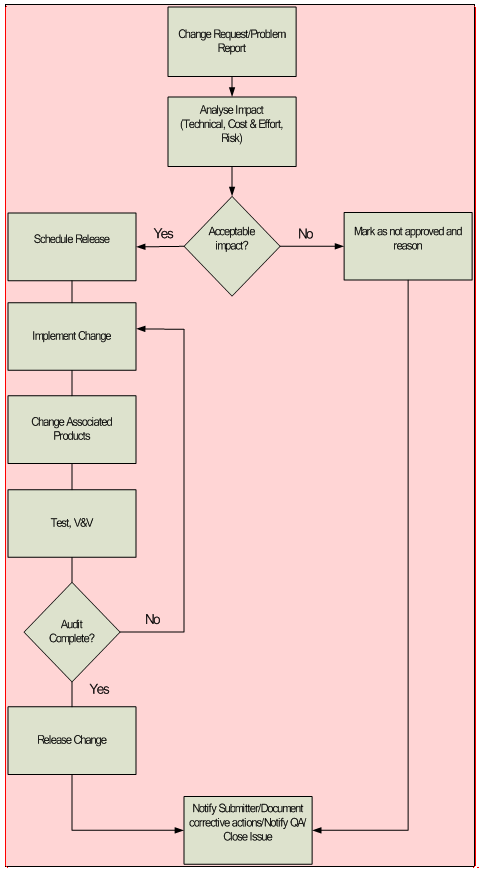
\includegraphics[scale=1.3]{./figures/changerequest.PNG}
\caption{Change/Problem Request process}
\end{figure}

\subsection{Software Deployment}
Process Definition see [N1 -- Chapter 9.1]

[F0E0?] additional project specific tasks

\begin{flushleft}
\tablefirsthead{}
\tablehead{}
\tabletail{}
\tablelasttail{}
\begin{supertabular}{|m{5cm}|m{9cm}|}
\hline
Role &
Responsibility\\\hline
Project Manager &
Development of the Software Deployment Plan

Monitoring and Approval of the software implementation\\\hline
Configuration Management Staff &
Build the product/software release, run regression tests, perform configuration audits and accounting, baseline and packaging the release.

Complete traceability including destination of the software.\\\hline
Implementation Team &
Preparation of the Version Description Document

Preparation of the Software Implementation Manual

Elaboration of the Software implementation Records\\\hline
Verifier &
Preparation of the Deployment Verification Report\\\hline
Quality Assurance Manager &
Independent reviewer of both the processes and the corresponding outcomes\\\hline
\end{supertabular}
\end{flushleft}



\begin{flushleft}
\tablefirsthead{}
\tablehead{}
\tabletail{}
\tablelasttail{}
\begin{supertabular}{|m{7cm}|m{7cm}|}
\hline
Quality mechanisms for Safe deployment &
Technique \& Approach\\\hline
Software Self-identification Mechanisms

(9.1.4.11) &
~
\\\hline
Error detection and/or avoidance mechanisms during deployment process (store, transfer, transmission and/or duplication of code operations)

(9.1.4.20) &
~
\\\hline
Automatic detection and safe management of incompatible components/versions

(9.1.4.8, 9.1.4.9) &
~
\\\hline
Provision of appropriate and accurate diagnostic information &
~
\\\hline
Safe Roll back capabilities  &
~
\\\hline
\end{supertabular}
\end{flushleft}


\subsection{Software Maintenance}
Process Definition see [N1 -- Chapter 9.2]

[F0E0?] additional project specific tasks


\begin{flushleft}
\tablefirsthead{}
\tablehead{}
\tabletail{}
\tablelasttail{}
\begin{supertabular}{|m{5cm}|m{9cm}|}
\hline
Role &
Responsibility\\\hline
Project Manager/Maintenance Manager (if different) &
Development of the Software Maintenance Plan

Preparation and maintenance of the project history register (already started at the beginning of the project)

Responsible for the Impact Assessment processes

Preparation of the software maintenance reports\\\hline
Configuration Management Staff &
Maintain complete software (CI) maintenance registers and complete and accurate modification reports\\\hline
CCB &
Approval of changes\\\hline
Implementation Team &
Implementation of changes

(as during the development process)\\\hline
Verifier

~
 &
Preparation of the software maintenance verification report

Verification activities, as during the development process\\\hline
Validator &
Validation activities, as during the development process\\\hline
Quality Assurance Manager &
Independent review processes\\\hline
\end{supertabular}
\end{flushleft}


\begin{flushleft}
\tablefirsthead{}
\tablehead{}
\tabletail{}
\tablelasttail{}
\begin{supertabular}{|m{7cm}|m{7cm}|}
\hline
Quality mechanisms for Maintainability &
Technique \& Approach\\\hline
Coding Standards &
~
\\\hline
Impact Assessment &
Before each implementation\\\hline
Data register and analysis &
Creation and maintenance of a project history register\\\hline
Design method selection mechanisms to facility the maintainability (7.3.4.28) &
~
\\\hline
Attenuation actions mechanisms (9.2.4.20) &
~
\\\hline
Mechanisms for evaluating the appropriateness of the methods, tools and techniques used in the modification/maintainability (part of 9.2.4.2 and CENELEC 126 phase 13) &
~
\\\hline
SW description mechanisms (7.1.1.1) &
~
\\\hline
Control mechanisms to guarantee the corrective actions adoption (6.6.4.1) &
~
\\\hline
Provision of appropriate and accurate modification management system (6.6.4.1) and configuration management system (6.5.4.12) &
~
\\\hline
\end{supertabular}
\end{flushleft}


\section{Structure \& Requirments}

\subsection{Project Organization}
In order to assure the EN 50128 SIL4 compliancy [Ref [N01] -- Chapter. 5.1], development process requires to clearly identify the Key Software Roles among the Work Packages and Tasks that have already been defined in the Full Project Proposal (Ref [D01]). It aims at ensure that all the personnel who have responsibilities for the software are organized, empowered and capable of fulfilling their responsibilities.



\subsubsection{Project structure diagram}
According to the CENELEC EN50128 Standard, the project organization is defined as follow, in order to manage a SIL4 software development process:

The preferred organizational structure for a SIL4 software Development activity encompasses several requirements defined in the Referenced Standard ({\S}5.1.2.10 in Ref [N01]),

In our project we will adopt this generic structure to the SCRUM methodology. In Scrum, new roles are defined and are mapped to the generic concept. In the following we assume the reader is familiar with Scrum terminology and Scrum methodology:



\begin{figure}
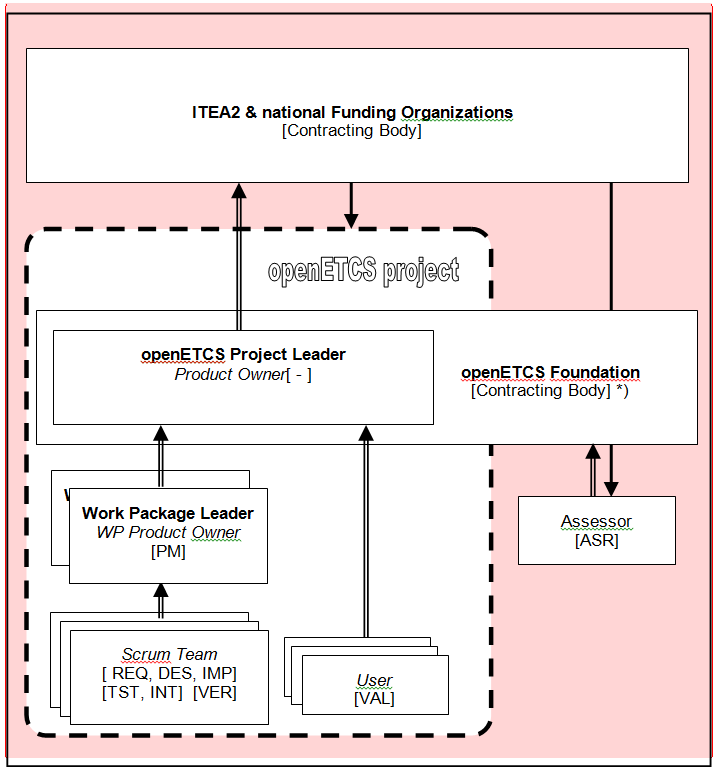
\includegraphics[width=\textwidth]{./figures/organization.png}
%\caption{??????}
\end{figure}



\paragraph{Scrum Roles in openETCS}
openETCS product owner role is fulfilled by the project lead of the EUPL openETCS project. As a product owner of openETCS, he is responsible for the openETCS product backlog.

The project is organized in a hierarchical manner. The project openETCS is split into work packages,. Same way the responsibility for the openETCS product is split to the WP leaders. In scrum, the WP leaders act as WP prduct owners for there respective part.

The WP product owner reports to the leader of the openETCS project. The contribution of all work packages builds the openETCS project.

The role of a workspace product owner nicely fits to the role of a project manager in the sense of EN50128.

Software development is done in Scrum teams. The team as a whole is responsible to reach the sprint targets and put all items to ``Done''. In each sprint, each of the Scrum Teams have to offer (or build) all necessary competences. The contribution of team members corresponds to the CENELEC roles ``Requirement Manager'' [RQM], ``Designer'' [DES], ``Implementer'' [IMP], ``Tester'' [TST], ``Integrator'' [INT] and ``Verifier'' [VER]. Teams need to take care competences for these roles are represented by the team members. However, during lifetime of the project, all team members may act in the different roles. 

In order not to jeopardize quality, we post the limitation an individual is not supposed to proof quality (i.e., review) of his own work. 

In practice, we request for each sprint a person shall not work in  the roles \{RQM, DES, IMP\} on one side and \{VER, INT, TST\} on the other side. 

Besides this restriction every member of the Scrum team can act in any of the roles provided by the team. Acting in various roles increases the competences of the teams over time and, at the same time, also quality and efficiency of team members.

According to CENELEC, the Validator [VAL] has a special responsibility. In our Scrum approach we use the role of the User to fulfill the Validator requirement.The role of the User is an essential component in scrum. In openETCS, naturally, the work packages product owner have to  act as User where appropriate.  In addition, active participation of representatives of the railway owners is required.

In practice, to fulfill the CENELEG Validator point of view, the User has to participate in Sprint Demonstrations and has to have a formal view on the quality aspects for the item. The User is invited also to have a closer look on the daily work of the Scrum teams.

Each Scrum team is supported by a scrum master. The scrum master represents the team at the work package product owner.

The Scrum Team size is recommended to be 6 members + scrum master.


\paragraph{Sprints in openETCS Scrum}
The schedule of the project is organized in sprints. Sprint, in general take 2 or 3 weeks of time. The frame schedule of the sprints will be defined by the openETCS product Owner and has to be aligned with eclipse release planning. Where necessary the sprint plans of different work packages might be synchronized, e.g., between Tools and the tool users. The project makes use of regular (weekly) Scrum of Scrum meetings. These meetings are meant to plan and improve the interaction of the work packages and to manage impediments.

Inside work packages the Work Package Product Owner is responsible for organizing Sprint Planning meetings, Sprint Review meetings and Sprint Retrospective according to Scrum.

The Scrum Master calls for a daily scrum meeting and represents the team in other activities.

Teams are responsible to complete all parts of implementation of their committed tasks. The result has to be documented at the end of the sprint in the sprint review for each item ``Done'' in the sprint. ``Done'' criteria are to be defined for each item in the sprint planning.



\paragraph{The Backlogs in openETCS Project}
The work in openETCS is split into several work packages. In general, the tasks of each work package build the work package backlog. 

The openETCS backlog defines priority of features for the project as a whole, i.e., workspace backlogs have to follow the priority of the project.

The priority of items in the backlogs is visible by the sequence in the backlog.

Items for daily work are managed in the task backlogs for the Scrum Teams. The backlogs are filled before starting the sprint in the sprint planning meeting. At sprint end the sprint result has to be reported back to the product backlog. This is one of the topics of the sprint review. 

The use of a professional backlog tool is highly recommended. The evaluation and selection of a tool is in responsibility of the project office. 


\paragraph{Aspects of Release Planning}
Releases are planned based on the Eclipse release schedule. In addition, the sprint schedule has to be aligned. At the end of each project sprint the outcome of the sprint is to be frozen as a set of parameters identifying a reproducible result of the project including all parts of the tool chain. 

Work package owners are responsible to make sure no untested results get committed to a release.


\paragraph{The role of the Assessor in openETCS}
In order to make the openETCS results easier useable by the industry after our initial project has finished the role of the Assessor [ASR] has to be implemented as an independently acting personality. With this role we follow the CENELEG proposal. We propose to use the openETCS foundation as a contractor for the Assessor. The Assessor will report to the openETCS foundation and, in the special situation of this ITEA 2 project, to ITEA 2.



\subsection{Documentation of Ecosystem}
https://github.com/openETCS/ecosystem/wiki/Documentation



\section{References and Abbreviation}
\subsection{Referenced Standards, Directives and Regulations}
\begin{flushleft}
\tablefirsthead{\hline
Nr. &
Document &
\centering\arraybslash Edition\\}
\tablehead{\hline
Nr. &
Document &
\centering\arraybslash Edition\\}
\tabletail{}
\tablelasttail{}
\begin{supertabular}{|m{1cm}|m{10cm}|m{3cm}|}
\hline
[N01] &
EN 50128 Railway applications -  Communication, signalling and processing systems -  Software for railway control and protection systems &
\centering\arraybslash 2011-06\\\hline
[N02] &
EN 50126 Railway applications - The specification and demonstraticn of Reliability, Availability, Maintainability and Safety (RAMS) &
\centering\arraybslash 2000-03\\\hline
[N03] &
EN 50129 Railway applications --  Communication, signalling and processing systems --  Safety related electronic systems for signalling &
\centering\arraybslash 2003-12\\\hline
[N04] &
EN~61508 Functional safety of electrical/electronic/programmable electronic safety-related systems &
{\centering 2010\par}

\centering\arraybslash Edition 2.0\\\hline
[N05] &
2008/57/EC -- Interoperability Directive &
\centering\arraybslash 17.06.2008\\\hline
[N06] &
2011/18/EU -- Interoperability Directive (change of annexes) &
\centering\arraybslash 01.03.2011\\\hline
[N07] &
2012/88/EU -- TSI CCS

technical  specification  for  interoperability  relating  to  the  control-command  and  signalling subsystems  of  the  trans-European  rail  system &
\centering\arraybslash 25.12.2012\\\hline
\end{supertabular}
\end{flushleft}



\subsection{Referenced Documents}
\begin{center}
\tablefirsthead{\hline
Doc. Nr.: &
Title &
Date\\}
\tablehead{\hline
Doc. Nr.: &
Title &
Date\\}
\tabletail{}
\tablelasttail{}
\begin{supertabular}{|m{2cm}|m{9cm}|m{3cm}|}
\hline
\centering [D01] &
Full Project Proposal openETCS &
11.04.2012\\\hline
\centering [D02] &
EN50128:2011 &
~
\\\hline
\centering [D03] &
TSI Subset 026 &
~
\\\hline
\centering [D04] &
TSI Subset 036 &
~
\\\hline
\centering [D05] &
TSI Subset 076 &
~
\\\hline
[SCRUM] &
Roman Pichler : Agile Product Management with Scrum &
22.3.2010

~
\\\hline
[SCRUM] &
Ken Schwaber and Mike Beedle : Agile Software Development with Scrum, Pearson Studium &
24.4.2008\\\hline
\centering FM &
Jean-Francois Monin : Understanding Formal Methods


&
17.1.2003\\\hline
\centering [ECLIPSE] &
t.b.d &
~
\\\hline
\end{supertabular}
\end{center}


\subsection{Abbreviations}
\begin{flushleft}
\tablefirsthead{\hline
Abb. &
Meaning\\}
\tablehead{\hline
Abb. &
Meaning\\}
\tabletail{}
\tablelasttail{}
\begin{supertabular}{|m{2cm}|m{12cm}|}
\hline
ASR &
Assessor\\\hline
CCS &
control-command and signalling subsystems  \\\hline
DES &
Designer\\\hline
ERTMS &
European Rail Traffic Management System

Train signaling system equipment based on a single Europe-wide standard for train control and command systems.\\\hline
ERA &
European Railway Agency\\\hline
ETCS &
European Train Control System

It is a signalling, control and train protection system designed to replace the many incompatible safety systems currently used by European railways\\\hline
EUPL &
European Union Public Licence\\\hline
EVC &
European Vital Control\\\hline
GSM-R

(train radio) &
Global System for Mobile Communications - Rail(way)

It is an international wireless communications standard for railway communication and applications.\\\hline
HR &
Highly Recommended\\\hline
HW &
Hardware\\\hline
IMP &
Implementer\\\hline
INT &
Integrator\\\hline
MVB &
Multifunction Vehicle Bus

It is a part of the Train Communication Network (TCN), and it takes part in digital operation in the train. MVB is the bus part in each coach, and the Wire Train Bus (WTB) allows connecting the MVB parts with the train control system.\\\hline
NA &
Not Applicable\\\hline
OBU &
On-Board Unit\\\hline
REQ &
Requirements Manager\\\hline
R\&D &
Research and Development\\\hline
SIL &
Safety Integrity Level\\\hline
SME &
~
\\\hline
SRS &
Software Requirements Specification\\\hline
SW &
Software\\\hline
SW-SIL &
Software-Safety Integrity Level (EN 50128:2011)\\\hline
TSI &
Technical Specification for Interoperability\\\hline
TST &
Tester\\\hline
VAL &
Validator\\\hline
VER &
Verifier\\\hline
V\&V &
Verification and Validation\\\hline
WP &
Work Package\\\hline
ASR &
Assessor\\\hline
ERTMS &
European Rail Traffic Management System

Train signaling system equipment based on a single Europe-wide standard for train control and command systems.\\\hline
ETCS &
European Train Control System

It is a signalling, control and train protection system designed to replace the many incompatible safety systems currently used by European railways\\\hline
GSM-R

(train radio) &
Global System for Mobile Communications - Rail(way)

It is an international wireless communications standard for railway communication and applications.\\\hline
MVB &
Multifunction Vehicle Bus

It is a part of the Train Communication Network (TCN), and takes part in digital operation in the train. MVB is the bus part in each coach, and the Wire Train Bus (WTB) allows connecting the MVB parts with the train control system.\\\hline
SIL &
Safety Integrity Level\\\hline
SW &
Software\\\hline
SW-SIL &
Software-Safety Integrity Level (EN 50128:2011)

~
\\\hline
FM &
Formal Methods\\\hline
IP &
Intellectual Property\\\hline
IP Clean &
No IP without permission in writing \\\hline
~
 &
~
\\\hline
\end{supertabular}
\end{flushleft}

\bigskip


\bigskip

\clearpage
\bigskip
\end{document}
